\chapter{Completed work}

In this section, we discuss our publications related to this
proposal, and emphasize our major contributions to the field. In short, we
discuss two models for hypernymy detection, and compare and contrast them other
work in the literature. We also discuss how one of these models can contribute
as one component in an end-to-end RTE system. Finally, we discuss our model for
the Lexical Substitution task, and why it improves upon prior work.

\section{Asym Model for Lexical Entailment (Roller et al., 2014)}
\label{sec:asym}

Most baseline similarity measures in distributional semantics, like cosine,
have the unfortunate property that they are symmetric: $\text{cosine}(a, b) =
\text{cosine}(b, a)$. While this often desirable, it
is a fatal flaw in any application involving lexical entailment: although {\em
girl} implies {\em child}, but the opposite does not hold. As such, attempts to
predict lexical entailment using solely symmetric measures will always fall
short.

This has been recognized widely in the
literature for some time, and numerous asymmetric, unsupervised similarity measures have been
proposed
\cite{weeds:2003:emnlp,zhitomirsky-geffet:2005:acl,clarke:2009:gems,kotlerman:2010:nle,santus:2013:thesis},
mostly inspired by the Distributional Inclusion Hypothesis (DIH), which
states that the contexts of a hypernym should be a superset of its hyponyms'.
However, their
performance tend to be lackluster \cite{clarke:2009:gems} or brittle
\cite{kotlerman:2010:nle}. This raises the question: are the measures just
overly sensitive to noise in distributional vectors, or is the Distributional
Inclusion Hypothesis fundamentally flawed? If the unsupervised are measures
are simply too sensitive to noise, perhaps using supervised techniques can
improve performance.  To this end, we propose Asym, a simple supervised model
that is inherent asymmetric and interpretable under the DIH
\cite{roller:2014:coling}. 

At its core, the model is inspired by the famous result of
\newcite{mikolov:2013:iclr}, who observed that vector subtraction can be used
to perform some kinds of analogical reasoning in some kinds of distributional
spaces: e.g., {\em king}$ - ${\em man}$ + ${\em woman}$ \approx ${\em queen}.
Interestingly, this vector subtraction approach reasonably models many
grammatical relationships (singular/plural, verb conjugations) and some limited
semantic relationships (gender, capital/country). Asym exploits this
behavior for the task of hypernymy and lexical relationship prediction.

The Asym model is a simple model which uses the {\em vector difference} between
the hypothesized hypernym-hyponym pair as input features to an off-the-shelf
classifier. For example, given a (unit normalized) distributional vector for
{\em animal} and a vector for {\em cat}, we use the vector
{\em animal}$ - ${\em cat} as a positive example, while the
vectors for {\em cat}$ - ${\em animal} and {\em animal}$ - ${\em sofa} are
inputted as negative examples. Additionally, we also give the {\em element-wise
squared difference vector} as features to the classifier. Formally, for a given
(hypernym, hyponym) pair of words, $(H, w)$, we compute the final feature space
defined as:
\begin{align*}
  A_i(H, w) & = H_i - w_i\\
  B_i(H, w) & = (H_i - w_i)^2\\
  \text{features}(H, w) & = \langle A; B\rangle,
\end{align*}
where $\langle A; B\rangle$ is the vector {\em concatenation}. This computation
is performed for all examples in our dataset, and then the features $(H, w)$
vector and the classification label are used to train a Logistic Regression
classifier.

One significant advantage of this model over other works is its direct
connection to the Distributional Inclusion Hypothesis: since our model uses the
vector difference as input, it naturally measures whether $H_i$ is
greater than $w_i$, effectively acting as a strict-subset measurement. The
difference-squared part of the input features measures whether they have a
large absolute difference, effectively capturing ``equal'' part of the
``less than or equal'' relation. As such, one interpretation of the model is a
kind of {\em Selective Distributional Inclusion Hypothesis}, which presupposes
that the DIH holds, but only in particular, relevant dimensions.

To evaluate our model, we train and measure accuracy of the Asym model on
two datasets in a variation of leave-one-out cross validation (LOOCV) and
measuring absolute accuracy. In this variation of LOOCV, we select one word
from the vocabulary in the datasets, and consider {\em all pairs} with that
word to be test pairs. The remainder of word pairs, which do not contain the
held out word, are treated as training pairs. This prevent classifiers from
simply memorizing that words like {\em animal} are more likely to be hypernyms.
This experimental setup is one of our core contributions to the literature, as
we were the first to recognize this problem and propose an experimental
setup which avoids it \cite{roller:2014:coling}. We revisit this issue in
more detail in Section~\ref{sec:lexmem}.

Since different types of distributional spaces exhibit different properties
\cite{pado:2007:cl}, we evaluate our model on two distributional
spaces which use a simple Bag-of-Words context.  The {\em Window-2 BoW} space
counts content words two words to the left and right of targets as contexts,
while the {\em Sentence BoW} space counts all content words within complete
sentence boundaries. Both spaces are reduced to 300 dimensions using the
Singular Value Decomposition \cite{landauer:1997:pr}.

We evaluate our model on two datasets. The first, {\bf LEDS}
\cite{baroni:2012:eacl}, contains 1385 hyponym-hypernym pairs as positive
examples and 1385 negative pairs which were generated by randomly shuffling the
positive examples. As such the model only contains hypernymy and random
relations, and we train a binary classifier. The second dataset is {\bf
BLESS} \cite{baroni:2011:gems}, which contains annotations of word relations
for 200 unambiguous, concrete nouns from 17 broad categories. Each noun is
annotated with its co-hyponyms, meronyms, hypernym and some random words.
Since there are four relations, we train four one-vs-all classifiers, and
predict the relation with the highest score; in this way, the model
actually learns to detect three different lexical relations, though this
was not our primary research interest at the time. We will reconsider this in
our proposed work.

We compare our model with two baselines: the first is a degenerate baseline,
which guesses false for the (balanced) LEDS dataset, and always
the most common label ({\em no-relation}) for BLESS. We also compare to the
model proposed in \newcite{baroni:2012:eacl}, which uses the {\em concatenation}
of the $H$ and $w$ vectors and trains an off-the-shelf polynomial Support
Vector Machine \cite{cortes:1995:ml}.

\begin{table}
  \centering
  \begin{tabular}{|lc|cc|}
    \hline
    {\bf Classifier} & {\bf Space} & {\bf LEDS} & {\bf BLESS}\\
    \hline
    Always guess false/no relation     &   -      & .50          & .46      \\
    \hline
    \cite{baroni:2012:eacl}            & Window 2 & .81          & .76      \\
    Asym \cite{roller:2014:coling}     & Window 2 & {\bf .85}    & {\bf .84}\\
    \cite{baroni:2012:eacl}            & Sentence & .78          & .73      \\
    Asym \cite{roller:2014:coling}     & Sentence & .82          & .80      \\
    \hline
  \end{tabular}
  \caption{Accuracy of Baroni et al. (2012) and Roller et al. (2014) on
  {\bless} and {\entailment}
  using different spaces for feature generation. Performance is measured as
  the average accuracy across all folds of the leave-one-out cross validation
  experiment.}
  \label{tab:asymresults}
\end{table}

Table~\ref{tab:asymresults} shows the results for our initial experiment.
First we notice that both models strongly outperform the degenerate baseline,
indicating there is some successful learning in the models. We also see that
the Window 2 space performs better than the Sentence space in all four
comparisons, indicating it is likely the task depends more heavily {\em
functional} properties of words than {\em topical} properties of words.

Finally, we see that the Asym model outperforms the model proposed by
\newcite{baroni:2012:eacl} in all four comparisons, indicating our architecture
has better lexical generalization.
Interestingly, we found that dropping the square-difference terms
severely hurt the performance of our model, emphasizing these features immense
importance. We will discuss more of why these features are so important in
Section~\ref{sec:lexmem}. Incidentally, at the same time that
\newcite{roller:2014:coling} was published, \newcite{weeds:2014:coling} and
\newcite{fu:2014:acl} also proposed supervised hypernymy models based on vector
difference, but neither of these employ the critical square-difference terms,
or adequately address the issue of lexical memorization.

We also test our interpretation of Asym as measuring a form of {\em Selective}
Distributional Inclusion. After training the model's parameters on the BLESS
dataset, we compare the model's learned hyperplane to the {\em context
vectors} obtained in the Singular Value Decomposition. We select the 500
features most similar to the model's hyperplane, and then extract a
distributional space limited to only these context items. If our Selective
Distributional Inclusion Hypothesis is true, we would expect these 500
dimensions to highly compliment existing similarity measures based on the
Distributional Inclusion Hypothesis. We note that we are directly comparing
unsupervised measures with a supervised model, and so this should only be
understood as an experiment about the {\em interpretation} of our model, not
its performance.

We measure every word pair's similarity using three similarity measures:
cosine, Clarke, and invCL. Cosine similarity acts as our scientific control, and
should {\em not} change substantially between the
original and selective spaces, while the others, which are
based on Distributional Inclusion, should. The second similarity measure,
{\em Clarke}, measures roughly what percentage of the hyponyms' mass is contained
within the hypernym \cite{clarke:2009:gems}:
\begin{equation*}
  \text{Clarke}(H, w) = \frac{\sum_i \min(H_i, w_i)}{\sum_i H_i};
\end{equation*}
The final similarity measure, {\em invCL}, extends Clarke to additionally
measure what percentage of the hypernym's mass is {\em not} contained within
the hyponym \cite{lenci:2012:starsem}, extending Clarke to roughly measure
{\em strict} containment:
\begin{equation*}
  \text{invCL}(H, w) = \sqrt{\text{Clarke}(H, w)(1 - \text{Clarke}(w, H))}.
\end{equation*}

We compute all three similarity measures across all the word pairs in BLESS,
and computed Mean Average Precision (MAP) across all pairs for each measure
and distributional space. Ideally, we should see that, compared to the original
space, the selective space has higher Clarke and invCL values
for hypernyms, and lower Clarke and invCL values for the other relations.
Table~\ref{tab:mapscores} shows the results of this experiment.

\begin{table}
  \centering
  \begin{tabular}{|l|cc cc||cccc|}
    \hline
    & \multicolumn{4}{c||}{Original Space} & \multicolumn{4}{|c|}{Selective Space}\\
    \hline\hline
    Measure        &\small \coord     &\small \hyper    &\small \mero      &\small \randomn  &\small \coord     &\small \hyper    &\small \mero      &\small \randomn  \\
    \hline
    cosine         &     .68     &     .20    &     .27     &     .27    &   .69      &    .20    &    .24     &    .28    \\
    Clarke         &     .66     &     .19    &     .28     &     .28    &   .55      &    .39    &    .24     &    .29    \\
    invCL          &     .60     &     .18    &     .31     &     .28    &   .42      &{\bf.58}   &    .24     &    .29    \\
    \hline
  \end{tabular}
  \caption{Mean Average Precision for the unsupervised measures before
  after selecting the top dimensions from the Asym model.}
  \label{tab:mapscores}
\end{table}

As expected, all measures except for cosine assign higher MAP values to
hypernyms than they did in the original space, though only invCL that ranks
hypernyms significantly higher than co-hyponyms.\footnote{Wilcoxon signed-rank
test, $p < .001$} We also see that the performance of our cosine baseline
remains relatively unchanged by the feature selection procedure, and that
the the Clarke and invCL measures have their co-hyponymy and meronomy
scores weakened. Altogether, this is evidence that the Asym measure is
indeed, conforming to our Selective Distributional Inclusion interpretation.


\section{Subsystem in complete RTE system (Beltagy et al., 2016)}
\label{sec:rtesubsystem}

Beyond showing that Asym is better able to improve performance on lexical
relationship datasets, we should also show that it can improve performance
in an end-to-end Recognizing Textual Entailment (RTE) system. Specifically, we compare Asym's performance
to a variety of lexical entailment classifiers which use a variety of
hand-engineered features and word lexicons.  These predictions made by lexical
entailment classifiers are used as to generate {\em logical rules}; an inference
engine based on Markov Logic Networks (MLNs) is then used to form predictions
about complete {\em sentential} entailment \cite{beltagy:2016:cl}.

To this end, we employ the Sentences Involving Compositional Knowledge (SICK)
dataset, which contains nearly 10k sentence pairs, evenly split between
training and test sets \cite{marelli:2014:semeval}. Sentence pairs were
extracted randomly image caption datasets, and then simplified and extended to
cover semantic issues like negation and quantifiers, and then manually
annotated as {\em entailing} (the antecedent implies the consequent), {\em
contradicting} (the antecedent implies the opposite of the consequent), or
neutral (neither of the above). Two examples from the dataset are shown in
Table~\ref{tab:sickexample}.

\begin{table}
  \centering
  \begin{tabular}{|ll|}
    \hline
    {\bf Label} & {\bf Antecedent/Consequent}\\
    \hline
    Entailing & A: Two teams are competing in a football match\\
    & C: Two groups of people are playing football\\
    \hline
    Contradicting & A: The brown horse is near a red barrel at the rodeo\\
    & C: The brown horse is far from a red barrel at the rodeo\\
    \hline
  \end{tabular}
  \caption{Example entailing and contradicting sentences from the SICK dataset.}
  \label{tab:sickexample}
\end{table}

To train the lexical entailment classifier, we extract {\em lexical pairs} from
the SICK dataset using a variation on Robinson Resolution \cite{robinson:1965:jacm}. The
full details are outside the scope of this document, but briefly, we employ
an off-the-shelf semantic parser called Boxer, which translates sentences into
First Order Logical formulas \cite{bos:2008:step}. We then use theorem proving
techniques in order to extract lexical rules which {\em must} be true in the dataset.
For example, given that ``The girl talks'' entails ``A girl speaks,'' we can
eliminate {\em girl} and automatically conclude that {\em talks} lexically
entails {\em speaks}.

Crucially, by knowing entailment decisions about the
entire sentences, and by performing unification over their logical structures,
we can use theorem proving to automatically label certain {\em atomic rules} as
entailing, contracting, or neutral. These atomic rules, like {\em talks entails speaks}, can
be interpreted as {\em lexical entailment pairs} for use in a lexical entailment
classifier. Most, but not all, pairs can be labeled automatically, and those
that cannot are manually annotated by two of the authors \cite{beltagy:2016:cl}.
The final result is a novel dataset of lexical entailment pairs, which we call
RRR (Robinson Resolution Rules), which we use to train and compare lexical
entailment classifiers.

We compare the performance of several existing lexical entailment
classifiers which employ a variety of hand-engineered features and lexicons
like WordNet.  Most of the hand-engineered features come from
\newcite{lai:2014:semeval}, and include things like Wordform features (e.g.,
do the words have the same lemma or Part-of-Speech?); WordNet features (e.g.,
are the words hypernyms or co-hyponyms in WordNet?); and Distributional
Similarity (e.g., cosine distance between two words in a distributional space).

We also present a novel extension of the real-valued distributional similarity
features, by {\em binning} cosines into ranges (e.g. 0.0--0.1, \ldots, 0.9--1.0)
to transform them into binary-valued features, after observing that
mid-similar terms (those with a cosine of $\sim.80$, like {\em cat} and {\em
animal}) were more likely entailments than those with high similarity
(cosine of $\sim.95$, like {\em cat} and {\em dog}). We found this binning
technique significantly improved the contribution distributional similarity
in feature-engineered lexical entailment classifiers.

Finally, we also compare to the Asym classifier trained on our new RRR dataset,
and on a variation of Asym which concatenates the Asym features with the
antecedent (LHS) and consequent (RHS) vectors, which we call Asym + Concat,
since it uses both the Asym features and the Concat (LHS+RHS) features. For
both the distributional similarity features, and the Asym models, we use two
distributional spaces: one which uses a BoW window of two words, and one based
on syntactic contexts.

We evaluate all of the lexical entailment classifiers listed above on two
variations of the task: Intrinsic accuracy, and RTE accuracy. In the Intrinsic
setup, the lexical entailment classifiers are evaluated on their performance on
the RRR dataset in a standard 10-fold cross-validation setup. In the RTE setup,
the classifiers are trained on items extracted from the training portion of the
RTE dataset, and then used as the sole source of lexical knowledge in a
complete RTE pipeline \newcite{beltagy:2013:starsem,beltagy:2016:cl}
to predict the test portion of the RTE dataset. This ensures we are actually
testing whether Asym is able to contribute in a rich RTE pipeline.

Table~\ref{tab:evallexical} shows performance of the various lexical entailment
classifiers on each of our evaluation settings. We also report a degenerate
baseline (always guess Neutral), and an upper baseline, which always gives gold
lexical entailment decisions. Note that this upper baseline on the RTE
task is {\em not} 100\%, due to a mixture of issues like parsing errors,
inference errors, and other issues in the RTE inference engine.

\begin{table}
\centering
\begin{tabular}{|lrr|}
    \hline
    {\bf Feature set} & {\bf Intrinsic} & {\bf RTE Test}\\
    \hline
    Always guess neutral & 56.6 & 69.3 \\
    Gold standard annotations&100.0 & 94.6 \\
    \hline
    Wordform only        & 57.4 & 70.4 \\
    Dist. Sim. only      & 68.8 & 76.7 \\
    WordNet only         & 79.1 & 84.2 \\
    Asym only            & 76.8 & 79.2 \\
    Asym + Concat        & 81.4 & 82.6 \\
    \hline
    All features         & 84.6 & 83.8 \\
    \hline
\end{tabular}
\caption{Accuracies for various Lexical Entailment classifiers on the RRR (Intrinsic) and SICK (RTE) datasets.}
\label{tab:evallexical}
\end{table}

In general, we find that Asym performs relatively well, even compared some of
the hand-engineered features proposed by \newcite{lai:2014:semeval}, indicating
that Asym is flexible and able to learn beyond just the LEDS and BLESS datasets.
Unsurprisingly, the classifiers which use only Wordform features or only
distributional similarity both perform much worse than the information-rich
WordNet features, or the more sophisticated Asym classifier.
We also notice that the classifier which combines Asym with the Concat
vectors performs substantially better than Asym does by itself, indicating
a need for additional study, which we will address in
Section~\ref{sec:hfeatures}.

Unsurprisingly, we find that the WordNet classifier does a bit better than the
others, which is expected given that WordNet is an information-rich resource,
and contains gold annotations about word relationships, rather than
distributional information.  Finally, we observe a classifier which combines
all of these features together does the best on the Intrinsic accuracy, but not
as strongly as WordNet on the end-to-end task; some of this can be attributed
to a handful of systematic differences between the training and test sets of
SICK.

We also perform a qualitative analysis to compare the Distributional Similarity
classifier with the Asym classifier. We manually inspect and compare the
predictions and errors made by each, and find that Asym does substantially
better at distinguishing hypernymy from co-hyponymy.  This is what we had hoped
to find, given the findings in Section~\ref{sec:asym}, and that cosine is known
to heavily favor co-hyponymy \cite{baroni:2011:gems}.  However, we also find
that cosine features are better at discovering synonymy, and that Asymmetric
frequently mistakes antonymy as an entailing. Additional qualitative analyses
comparing models are available in \newcite{beltagy:2016:cl}.

\section{H-Features for Hypernymy Classification (Roller and Erk, 2016b)}
\label{sec:hfeatures}

In the previous sections, we saw that the Asym classifier is able to reasonably
learn to classify word pairs as hypernymy and non-hypernymy, and that is able
to contribute in an end-to-end RTE system. However, we also saw in our
RTE experiments that Asym can be improved upon by simply concatenating the Asym
difference vectors with vectors for the LHS and the RHS (which we call Concat).
In this section, we discuss some of the strengths and weaknesses of the Concat
model, and how these relate to the Asym model. We then propose a novel
classification model which combines and extends the strengths of all these
models using an iterative procedure similar to Principal Component Analysis
(PCA).

\subsection{Concerning Lexical Memorization}
\label{sec:lexmem}

After the publication of several supervised distributional models of hypernymy
\cite{baroni:2011:gems,fu:2014:acl,roller:2014:coling,weeds:2014:coling},
another study followed questioning whether these models truly learn to predict
relationships. \newcite{levy:2015:naacl} hypothesized that each of these models
is learning about {\em prototypicality}, or simply what a prototypical
hypernym looks like. For example, after learning that ``cat is an animal''
and that ``dog is an animal,'' a prototypicality classifier may also conclude
that ``sofa is an animal.'' That is, a prototypicality classifier will
simply learn that {\em animal} is usually a hypernym, and will always
predict this way.

The crux of the argument is explained analytically by
\newcite{levy:2015:naacl}, and hinges on observing that many of the models from
the literature use {\em linear} classifiers. Thus, consider a
classifier which takes the concatenation of the vectors $\wordpair$ learns a
hyperplane $\hat p$ to make its prediction. Then the hyperplane $\hat p$ can
also be viewed as a concatenation of two vectors:
\begin{align*}
  & \hat p^\top \langle H, w\rangle\\
  & = \protopair^\top \wordpair\\
  & = \hat H^\top H + \hat w^\top w
\end{align*}
This analysis shows that, when the hyperplane $\hat p$ is evaluated on a novel
pair, it lacks any form of direct interaction between $H$ and $w$ like the
inner product $H^\top w$, but rather only learns to capture the notion of
hypernymy through $\hat H$ and $\hat w$, the {\em prototypicality vectors}.
Without having some form of interaction, this Concat classifier has no way
of estimating the relationship between the two words. Furthermore, a linear classifier
which uses the Diff vectors as input ($H - w$) will also have this flaw,
since the hyperplane $\hat p$ can be analyzed in this same fashion.

In their work, \newcite{levy:2015:naacl} back up this analysis with experimental
evidence, showing that when the training/testing set is constructed to
ensure that no lexical items are shared between the training and test sets
(a variant of the experiments of \newcite{roller:2014:coling}), the performance
of several classifiers, like \newcite{baroni:2012:eacl} and
\newcite{weeds:2014:coling}, drop dramatically. \newcite{levy:2015:naacl} also
propose a new model which incorporates the inner product term, which
outperforms other models on several data sets.
Interestingly, Asym does {\em not} suffer this fundamental flaw: although it uses the
vector difference vectors as features, it also uses the {\em square-difference
vectors} as input. Crucially, by the Law of Cosines, we can see that these
square-difference features provide it these crucial inner product term:
\begin{align*}
  & \sum_i (H_i - w_i)^2\\
  & = \sum_i H_i^2 + w_i^2 - 2({H}_i{w}_i)\\
  & = H^\top H + w^\top w - 2{\bf H^\top{w}}
\end{align*}
This explains our observation in Section~\ref{sec:asym} that, without these
square-difference terms, performance drops substantially.

Nonetheless, this raises a concern about what the difference terms $H - w$
actually provide. We propose a qualitative experiment which explains, in
clear terms, why these terms are valuable, and leads to another model to
extend this behavior. For simplicity, we focus our analysis on the linear
Concat classifier, which exhibits the same behavior as Diff, but in a
more obvious way.

In our qualitative experiment, we train a linear Concat classifier using
syntactic distributional vectors on four separate data sets. We then analyze
the trained models by comparing their hyperplanes to the {\em context vectors}.
That is, we explicitly compare the $\hat H$ vector to the syntactic context
matrix $C$ in Equation~\ref{eqn:svd}. This is a radically
different view of than the prototypicality hypothesis of
\newcite{levy:2015:naacl}: rather than learning a prototype of hypernymy, our
interpretation is that the Concat and Diff models learn to act as {\em feature
detectors}, which identifies features (i.e. syntactic contexts), which are
useful in identifying hypernymy.  This interpretation and corresponding
experiment is a one of our core contributions to the literature.

We train the model on four data sets: LEDS, BLESS, Medical, and TM14. LEDS and BLESS
were also used in the Asym experiments, and are datasets covering hypernymy and
non-hypernymy relations. Medical is a dataset of pairs of medical words and
entailment labels, and was farmed using Information Extraction techniques
\cite{levy:2014:conll}. Finally, TM14 contains many varied word relations (like
cause-effect, agent-object) which are annotated with entailment decisions by
\newcite{turney:2015:nle}.

\begin{table}
\begin{center}
  \begin{small}
  \begin{tabular}{|llll|}
    \hline
    LEDS & BLESS & Medical & TM14\\
    \hline
      nmod:such\_as+animal             &  nmod:such\_as+submarine          &  nmod:such\_as+patch              &  amod+desire                        \\
      acl:relcl+identifiable           &  nmod:such\_as+ship               &  nmod:such\_as+skin               &  amod+heighten                      \\
      nmod:of\depinv+determine         &  nmod:such\_as+seal               &  nmod:including+skin              &  nsubj\depinv+disparate             \\
      nmod:of\depinv+categorisation    &  nmod:such\_as+plane              &  nmod:such\_as+tooth              &  nmod:such\_as+honey                \\
      compound+many                    &  nmod:such\_as+rack               &  nmod:such\_as+feather            &  nmod:with\depinv+body              \\
    \hline
  \end{tabular}
  \end{small}
\end{center}
\caption{Most similar contexts to the $\hat H$ hyperplane learned by a Concat classifier.}
\label{tab:ctxsim}
\end{table}

Table~\ref{tab:ctxsim} shows the five contexts most similar to the hyperplane
learned from each of the four datasets, and immediately explains why these models
perform strongly.  Nearly all of the contexts preferred by the model take the
form of Hearst patterns \cite{hearst:1992:coling,snow:2004:nips}.  The most
recognizable and common pattern learned is the ``such as'' pattern, as in
``animals such as cats''.  These patterns have been well known to be indicative
of hypernymy for over two decades. Other interesting patterns are the
``including'' pattern (``animals including cats'') and ``many'' pattern (``many
animals''). Although we list only the five most similar context items for the
data sets, we find similar Hearst Pattern type contexts continue to dominate
the list for the next 30-50 items.

Altogether, it is remarkable that the model identified these patterns using
{\em only} distributional vectors and only the positive/negative example pairs.
Since the model can be interpreted as a sort of {\em feature detector}, we
call this model the H-feature Detector Model.
We now show how these H-features
can be improved using an iterative procedure similar to Principal Component
Analysis.

\subsection{The H-Feature Detector Model}

Knowing that the Concat classifier acts primarily as a feature detector, we ask
whether this can be combined with similarity-based insights of models like
Asym. To this end, we propose a novel model which exploits the H-feature
Detector model, extends its modeling power, and also adds in features for
general similarity and distributional inclusion.

The model works through an iterative procedure similar to Principal Component
Analysis (PCA). Each iteration repeatedly trains a Concat classifier under the
assumption that it acts as a feature detector, and then explicitly {\em discards}
this information from the distributional vectors. By training a new feature
detector on these modified distributional vectors, we can find additional
features indicative of entailment which were not captured by the first
classifier. This is similar to how in Principal Component Analysis, the
second principal component is computed after the first principal component
has been accounted for.

The main insight is that after training some feature detector using Concat,
we can {\em remove} this feature from the distributional vectors through
the use of {\em vector projection}.
Formally, the vector projection of $x$ onto
a vector $\hat p$, $\text{proj}_{\hat p}(x)$ finds the {\em component} of $x$
which is in the direction of $\hat p$,
\begin{equation*}
  \text{proj}_{\hat p}(x) = \left(\frac{x^\top\hat p}{\|\hat p\|}\right)\hat p.
\end{equation*}
Figure~\ref{fig:vecproj} gives a geometric illustration of the vector
projection. If $x$ forms the hypotenuse of a right
triangle, $\text{proj}_{\hat p}(x)$ forms a leg of the triangle. This also
gives rise to the {\em vector rejection}, which is the vector forming the third
leg of the triangle. The vector rejection is orthogonal to the projection, and
intuitively is ``leftover'' vector after the projection has been removed:
\begin{equation*}
  \text{rej}_{\hat p}(x) = x - \text{proj}_{\hat p}(x).
\end{equation*}

\begin{figure}
  \begin{center}
  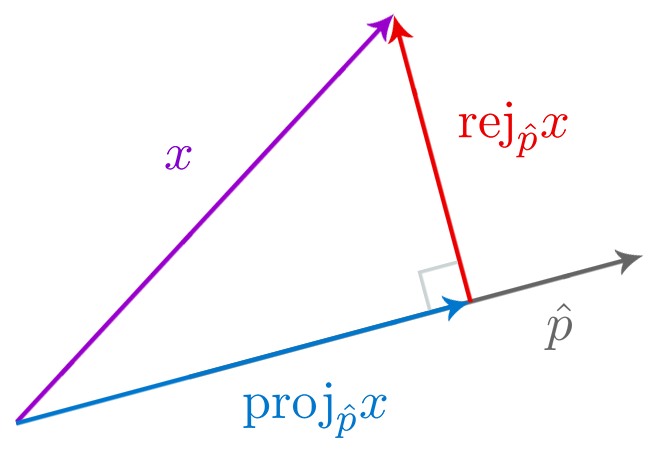
\includegraphics[width=0.30\textwidth]{figures/vecproj}
\end{center}
\caption{A vector $\hat p$ is used to break $H$ into two orthogonal components,
its projection and the rejection over $\hat p$.}
\label{fig:vecproj}
\end{figure}

Using the vector rejection, we take a learned H-feature detector $\hat p$,
and remove these features from each of the data points. That is, for every data
point $\langle H, w\rangle$, we replace it by its vector rejection and rescale
it to unit magnitude:
\begin{align*}
  H' & = \text{rej}_{\hat p}(H) / \|\text{rej}_{\hat p}(H)\|\\
  w' & = \text{rej}_{\hat p}(w) / \|\text{rej}_{\hat p}(w)\|
\end{align*}
A new classifier trained on the $\langle H', w'\rangle$ data must learn
a very different decision plane than $\hat p$, as $\hat p$ is no longer present
in any data points. This new classifier will perform strictly worse than the
original, otherwise the first classifier would have learned this hyperplane.
Nonetheless, it will be able to learn {\em new} H-features which the
original classifier was unable to capture. By repeating this process several
times, we can find several H-feature detectors, $\hat p_1, \ldots, \hat p_n$.

In each iteration $i$ of the procedure, we generate a four-valued feature vector
$F_i$, based on the H-feature detector $\hat p_i$. Each
feature vector contains (1) the similarity of $H_i$ and $w_i$ (before projection);
(2) the H-feature detector
$\hat p_i$ applied to $H_i$; (3) the H-feature detector $\hat p_i$ applied to $w_i$; and
(4) the difference of 2 and 3.
\begin{align*}
  & F_i(\langle H_i, w_i\rangle, \hat p_i)\\
  & \qquad = \langle H_i^{\top}w~~;~~H_i^\top\hat p_i~~;~~w_i^\top\hat p_i~~;~~H_i^\top\hat p_i - w_i^\top\hat p_i\rangle
\end{align*}
These four ``meta''-features capture all the benefits of the H-feature
detector (slots 2 and 3), while addressing Concat's issues with
similarity arguments (slot 1) {\em and} distributional inclusion (slot 4).

The union of all the feature vectors $F_1, \ldots, F_n$ from repeated iteration form a
$4n$-dimensional feature vector which we use as input to another classifier.
This classifier is trained on the exact same training data as each of the
individual Hearst Pattern detectors, so the procedure only acts as a method of
feature extraction. We use an SVM with an RBF-kernel, as we found it to work
best, though several nonlinear classifiers also perform well.

\begin{table}
\centering
\begin{small}
\begin{tabular}{|l|rrrr|}
  \hline
  Model            &      LEDS   &      BLESS  &      Medical  &      TM14   \\
  \hline
  \hline
  \multicolumn{5}{|c|}{Linear Models}\\
  \hline
  Cosine only (Baseline)              &      .787   &      .208   &      .168     &      .676   \\
  Concat                              &      .794   &      .612   &      .218     &      .693   \\
  Diff \cite{weeds:2014:coling}       &      .805   &      .440   &      .195     &      .665   \\
  Asym \cite{roller:2014:coling}      &      .865   &      .510   &      .210     &      .671   \\
  %Concat+Diff                        &      .801   &      .604   &      .224     &      .703   \\
  Asym + Concat \cite{beltagy:2016:cl}&      .843   &  {\bf.631}  &      .240     &      .701   \\
  \hline
  \multicolumn{5}{|c|}{Nonlinear Models}\\
  \hline
  RBF                                         &      .779   &      .574   &      .215     &      .705   \\
  Ksim \cite{levy:2014:conll}                 &      .893   &      .488   &      .224     &  {\bf.707}  \\
  H-Feature Detector \cite{roller:2016:emnlp} &  {\bf.901}  &  {\bf.631}  &  {\bf.260}    &      .697   \\
  \hline
\end{tabular}
\end{small}
\caption{Mean F1 scores for each model and data set.}
\label{tab:hfeatureresults}
\end{table}

We compare our H-feature detector model to several existing and alternative
baselines from the literature. Namely, we include a baseline Cosine classifier,
which only learns a threshold which maximizes F1 score on the training set;
three linear models of prior work, Concat, Diff and Asym; and the RBF and Ksim
models found to be successful in \newcite{kruszewski:2015:tacl} and
\newcite{levy:2015:naacl} respectively. We also include
Asym + Concat, which was used in \newcite{beltagy:2016:cl}. We cannot include a
additional comparisons like Ksim+Asym, because Ksim is based on a custom SVM
kernel which is not amenable to combinations.

Table~\ref{tab:hfeatureresults} the results across all four data sets for all
of the listed models. Our H-Feature model improves
significantly\footnote{Bootstrap test, $p<.01$.} over Concat in the LEDS, BLESS
and Medical data sets, indicating the benefits of combining these the aspects
of similarity and distributional inclusion with the H-feature detectors of
Concat.  The Asym + Concat classifier also improves over the Concat baseline,
further emphasizing these benefits. Our H-feature model performs approximately
the same as Ksim on the LEDS and TM14 data sets (no significant difference),
while significantly outperforming it on BLESS and Medical data sets.



\section{Lexical Substitution (Roller and Erk, 2016a)}
\label{sec:pic}

\begin{figure}
  \centering
  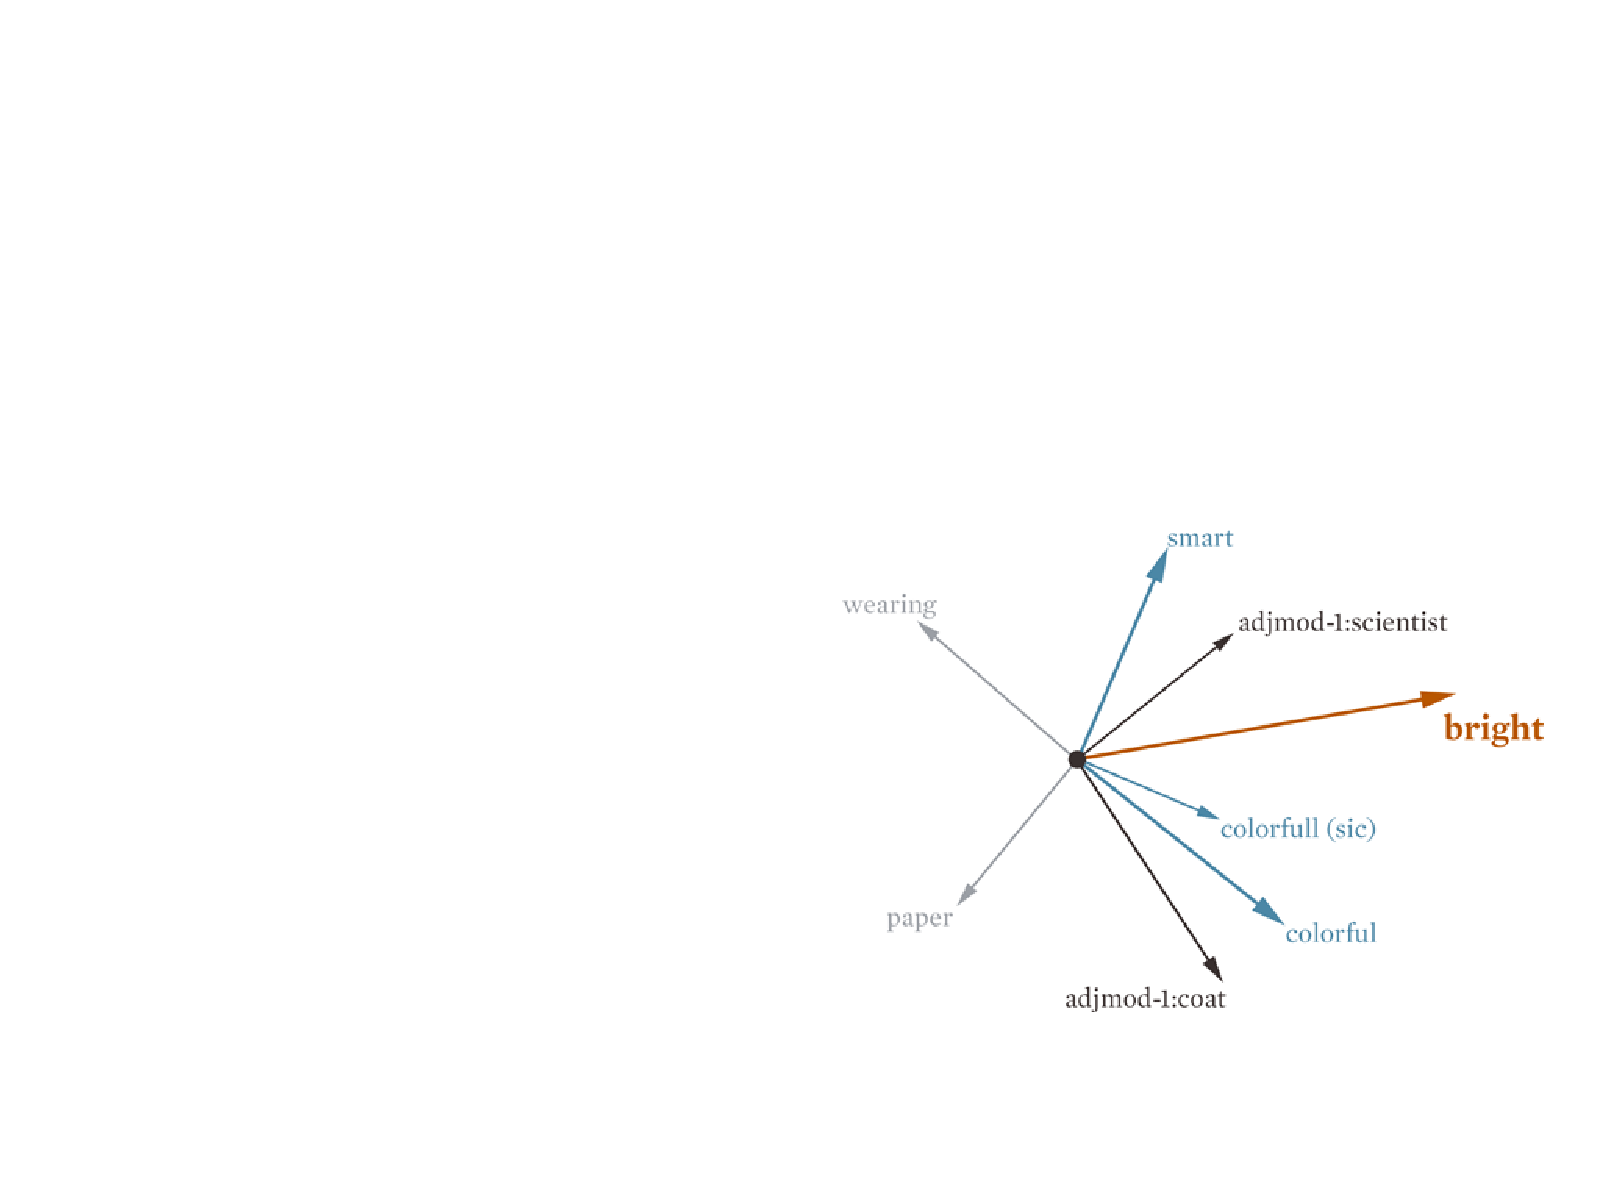
\includegraphics[width=0.5\textwidth]{figures/substitution}
  \caption{Caption here.}
  \label{fig:substitution}
\end{figure}

In this last section of our work, we switch over to our efforts on the Lexical
Substitution (LexSub) task. In the Lexical Substitution task, we are given
a sentence and target word, and must choose possible substitutes from the
entire vocabulary which preserve the meaning of the sentence.
As described in Section~\ref{sec:lexsub}, we view
LexSub as a proxy which captures a wide degree of lexical entailments {\em in
context}.

We propose a new measure, which extends
a previously successful, simple model to estimate the appropriateness of a
lexical substitute. As a introduction point for our measure, we review the work
of \newcite{melamud:2015:vsm}, which introduced several unsupervised measures
for word similarity in context: namely \balAddCos and \addCos. The main insight
of these unsupervised measures is the use of {\em context vectors}, related
to the insights discussed in Section~\ref{sec:lexmem}. Crucially, the models
of \newcite{melamud:2015:vsm} depend on syntactic context vectors, which
have been found more successful than just BoW measures in the literature
\cite{erk:2008:emnlp,dinu:2010:emnlp,thater:2010:acl,vandecruys:2011:emnlp}.
We note that these models are {\em not} the state of the art,
\cite{melamud:2015:naacl,melamud:2016:conll} but perform competitively while
remaining simple, extensible, and highly interpretable.

In the work of \newcite{melamud:2015:vsm} and others, substitutes are modeled
using a mixture of {\em out-of-context similarity} and {\em in-context
appropriateness}. The out-of-context similarity uses standard distributional
semantics cosine similarity (Equation~\ref{eq:cos}) in order to estimate how similar
the target is to the substitute, and remains fixed regardless of the sentential
context.  For this reason, this out-of-context (OOC) similarity is also used as
a baseline in the literature.

The in-context appropriateness attempts to directly model
whether a proposed substitute fits in the given sentential context. That is, if
one replaces the target with the substitute directly, would a reader still
consider this word {\em selectionally} agrees in the sentence. For example,
the in-context measures will give a low score for {\em dog purrs}, since dogs
usually do not purr.
To this end, it assumes the sentence is parsed, so that we have the full set of
syntactic neighbors of the target, $C$. Each of the context vectors
corresponding to elements of $C$ are then evaluated for their fit with the
proposed substitute, as illustrated in Figure~\ref{fig:syn}. For a given target
$t$, substitute $s$ and context $C$, the final \addCos~score is given as
\begin{equation}
  \text{addCos}(s|t,C) = \text{cosine}(s, t) + \sum_{c\in C} \text{cosine}(s, c).
\end{equation}
The model can be intuitively understood using the diagram in
Figure~\ref{fig:substitution}. For a given target ``bright,'' we will choose
the substitute (``smart'' or ``colorful'') which is {\em closer} to the
given context. If the context is ``scientist'' as in ``bright scientist,''
we will shift our prediction away from ``colorful'' and closer to ``smart,''
and vice versa for ``bright coat.'' This remains one of the simplest successful
models of Lexical Substitution to date. \newcite{melamud:2015:vsm} also consider
variants of this measure, including {\em balAddCos}, which equally
weights the out-of-context similarity with the in-context appropriateness:
\begin{equation}
  \text{balAddCos}(s|t,C) = \text{cosine}(s, t) + \frac{1}{|C|}\sum_{c\in C} \text{cosine}(s, c).
\end{equation}

In our work, we propose a new measure, called Probability-in-Context (PIC),\footnote{PIC is not strictly a probability measure; the name is a backronym for the purpose of the paper's title.}
which estimates the appropriateness of a substitute in a given context
\cite{roller:2016:naacl}.  Similar to \balAddCos, the measure has two
equally-weighted, independent components measuring the appropriateness of the
substitute for both the target and the context, each taking the form of a
softmax:
\begin{equation}
  \begin{aligned}
  \mbox{PIC}(s | t, C) &\propto P(s | t) \times P(s | C)\\
  P(s | t) &= \frac{1}{Z_t}\exp\left\{s^\top t\right\}\\
  P(s | C) &= \frac{1}{Z_C}\exp\left\{\sum_{c\in C}s^\top\left[Wc + b\right]\right\},
  \end{aligned}
  \label{eqn:pic}
\end{equation}
where the $Z_t$ and $Z_C$ are normalizing constants.
Our model differs from {\em balAddCos} in one major way: we base our similarity
estimates using the {\em unnormalized} inner product $s^\top t$ and $s^\top c$,
rather than normalized cosine similarities. We also introduce two additional
parameters, $W$ and $b$, which act as a simple linear transformation over the
original context vectors. These parameters are learned from the original
corpus, and serve only to tune how the fixed distributional vectors act in this
alternative objective function.

To identify the contribution of this parameterization versus the softmax
objective, we also introduce to a non-parameterized PIC ({\em nPIC}), which
does not contain the extra parameters:
\begin{equation}
  \begin{aligned}
  \mbox{nPIC}(s | t, C) &= P(s | t) \times P_n(s | C)\\
  P_n(s | C) &= \frac{1}{Z_n}\exp\left\{\sum_{c\in C}s^\top c\right\}
  \end{aligned}
  \label{eqn:npic}
\end{equation}

We compare our model to that of an out-of-context baseline (cosine) and the
{\em addCos} and {\em balAddCos} models of \newcite{melamud:2015:vsm}, which
outperformed other prior work at the time of its publication. We compare the
models on three data sets: SE07, the original LexSub data set
\cite{mccarthy:2007:semeval} which was explicitly developed to capture polysemy;
Coinco, a recent LexSub data set which contains substitutes for all content
words in a small corpus \cite{kremer:2014:eacl}; and TWSI2, which was developed
to be a large collection of lexical substitutes from a diverse corpus
\cite{biemann:2012:lrec}. We measure performance in Mean Precision@1, which
measures whether our best proposed substitute is contained within the set of gold
substitutes provided by annotators. In all models, we exclude any words sharing
the same lemma as the target, e.g. if the target is ``barking'' we do not
propose ``bark.''

\begin{table}
\begin{center}
\begin{tabular}{|l|r|r|r|}
  \hline
  {\bf Measure} & {\bf SE07} & {\bf Coinco} & {\bf TWSI2}\\
  \hline\hline
  %\multicolumn{4}{|c|}{Candidate Ranking (GAP)}\\
  %\hline
  %\ooc               &     44.2   &     44.5  &     57.9       \\
  %\addCos            &     51.2   &     46.3  &     62.2       \\
  %\balAddCos         &     49.6   &     46.5  &     61.3       \\
  %\hline
  %\ourmeas           &     51.3   &     46.4  &     61.8       \\
  %\ourmeasparam      & {\bf52.4}  & {\bf48.3} & {\bf62.8}      \\
  %\hline\hline
  %\multicolumn{4}{|c|}{All-Words Ranking (Mean Precision@1)}\\
  %\hline
  Cosine (OOC Baseline)                    &     11.7   &    10.9   &      9.8       \\
  addCos                                   &     12.9   &    10.5   &      7.9       \\
  balAddCos                                &     13.4   &    11.8   &      9.8       \\
  \hline
  nPic                                     &     17.3   &    16.3   &     11.1       \\
  PIC                                      & {\bf19.7}  &{\bf18.2}  & {\bf13.7}      \\
  \hline
  %\hline
  %\multicolumn{4}{|c|}{All-Words Ranking (Mean Precision@3)}\\
  %\hline
  %\ooc               &     9.7    &     8.6   &     7.0       \\
  %\addCos            &     9.0    &     7.9   &     6.1       \\
  %\balAddCos         &     9.8    &     9.1   &     7.4       \\
  %\hline
  %\ourmeas           &    13.1    &    12.1   &     7.9       \\
  %\ourmeasparam      &{\bf14.8}   &{\bf13.8}  &{\bf10.1}      \\
  %\hline
\end{tabular}
\end{center}
\caption{Lexical Substitution results for the all-words prediction task, measured
in Mean Precision@1.}
\label{tab:lexsub}
\end{table}

Table~\ref{tab:lexsub} contains results for all measures across all datasets.
We observe that PIC outperforms all other models by a significant
margin,\footnote{Wilcoxon signed-rank test, $p < 0.01$} including a relative
30\% improvement over \balAddCos in SE07 and Coinco. The nPIC also improves
substantially over the other baselines, indicating we gain benefit both from
the new objective function and the additional parameterization.  We next
strive to understand why both measures have a clear improvements over the
baseline models.

\begin{table*}[t]
  \begin{center}
  \begin{tabular}{|cccc|}
    \hline
    \ooc             & \balAddCos            & \ourmeas         & \ourmeasparam\\
    \hline\hline
    \multicolumn{4}{|c|}{You can sort of challenge them well, did you}\\
    \multicolumn{4}{|c|}{{\bf really} know the time when you said yes?}\\
    \hline\hline
    {    trully              } & {    proably             } & {    realy               } & {\bf actually            } \\
    {\bf actually            } & {    trully              } & {\bf truly               } & {\bf truly               } \\
    {    actaully            } & {    acutally            } & {\bf actually            } & {    already             } \\
    {    acutally            } & {    actaully            } & {    hardly              } & {    barely              } \\
    {    proably             } & {    probaly             } & {\bf definitely          } & {    just                } \\
    \hline
  \end{tabular}
  \end{center}
  \caption{Example where the \ourmeasparam~performs strictly better than other models. The target word and correct answers
  are bolded.}
  \label{tab:cherry}
\end{table*}

We characterize the models using a cherry-picked example,
given in Table~\ref{tab:cherry}. Although this example does not perfectly illustrate
the Lexical Substitution task, it does well at giving intuition as to why our
models perform better. We see that all four measures
tend to pick excellent substitutes which {\em semantically} agree with the
original target. However, the cosine and {\em balAddCos} models have a large number of
misspelled works in their list, while the nPIC and PIC measures contain
mostly correct spellings. This is because, somewhat surprisingly, the {\em
length} of the distributional vectors correlates strongly with the {\em
unigram} statistics of the word \cite{wilson:2015:arxiv}.
Therefore, by using the unnormalized inner
product, rather than cosine, our model naturally incorporates unigram priors,
allowing it to downweight rare, similar words. Indeed, a quantitative analysis
of the $W$ and $b$ parameters finds that they additionally exaggerate this
unigram bias \cite{roller:2016:naacl}.
Intuitively, it seems natural that unigram biases should hold a strong role in
Lexical Substitution, and that our model should wish to exploit this
information.


